\documentclass[a4paper, 12pt]{report}

\makeatletter
\renewcommand{\@seccntformat}[1]{}
\makeatother

\renewcommand{\labelenumii}{\arabic{enumi}.\arabic{enumii}.}

\renewcommand{\theenumi}{\arabic{enumi}.}
\renewcommand{\labelenumi}{\arabic{enumi}.}
\renewcommand{\theenumii}{\arabic{enumii}.}
\renewcommand{\labelenumii}{\arabic{enumi}.\arabic{enumii}.}
\renewcommand{\theenumiii}{\arabic{enumiii}}
\renewcommand{\labelenumiii}{\arabic{enumi}.\arabic{enumii}.\arabic{enumiii}.}

\usepackage{cmap}
\usepackage[T2A]{fontenc}
\usepackage[utf8]{inputenc}
\usepackage[english, russian]{babel}
\usepackage{hyperref}

\usepackage{graphicx}
\graphicspath{{./images/}}

\author{ГАПОУ БАСК}

\title{Windows server. Практическая работа №1}

\date{\today}

\begin{document} %
	
	\maketitle
	\clearpage

	\section{Комплектация задания}

	\begin{enumerate}
		\item Гипервизор VMware
		\item Виртуальная машина с ОС Windows 10
		\item Виртуальная машина с ОС Windows Server 2019
	\end{enumerate}

	\section{Задачи}
	
	\subsubsection{Настройка SRV1}
	
	\begin{enumerate}
		\item Базовая настройка
		\begin{enumerate}
			\item Переименовать компьютер в SRV1;
			\item Установить первый возможный адрес из адресного пространства 10.10.10.0/24;
			\item Обеспечьте работоспособность протокола ICMP (для использования команды ping).
		\end{enumerate}
		\item Active Directory
		\begin{enumerate}
			\item Сделайте сервер контроллером домена bask-rb.ru.
		\end{enumerate}
		\item DHCP
		\begin{enumerate}
			\item Настройте протокол DHCP для автоконфигурации клиентов – в качестве диапазона выдаваемых адресов используйте все не занятые серверами адреса в подсети.
		\end{enumerate}
	\end{enumerate}

	\subsubsection{Настройка CLI1}

	\begin{enumerate}
		\item Базовая настройка
		\begin{enumerate}
			\item Переименовать компьютер в CLI1;
			\item Настройте динамическую конфигурацию IP;
			\item Авторизуйтесь в контролере домена bask-rb.ru.
		\end{enumerate}
	\end{enumerate}

	\clearpage
	
	\section{Решение}
	
	\subsection{Настройка локальной сети VMware}
	
	По умолчанию VMware создает одну NAT сеть между виртуальными машинами и сервером. Нам же нужно создать локальный сегмент между CLI1 и SRV1.
	
	Нажмите правой кнопкой мыши на виртуальную машину, выберете в контекстном меню "Параметры..."
	
	\begin{figure}[h]
		\center{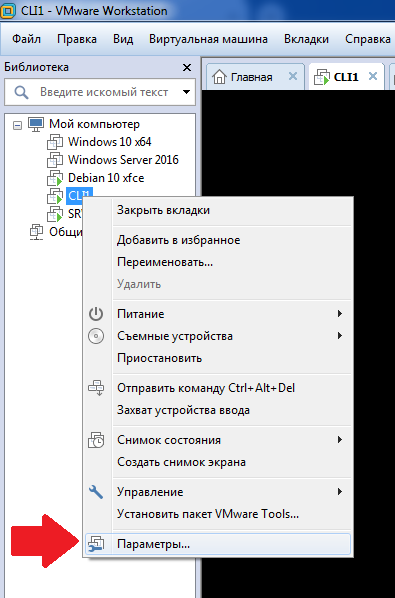
\includegraphics[scale=0.6]{_1}}
		\label{fig:image}
	\end{figure}

	\clearpage

	Откройте вкладку "Сетевой адаптер", нажмите на "Сегменты локальной сети...".

	\begin{figure}[h]
		\center{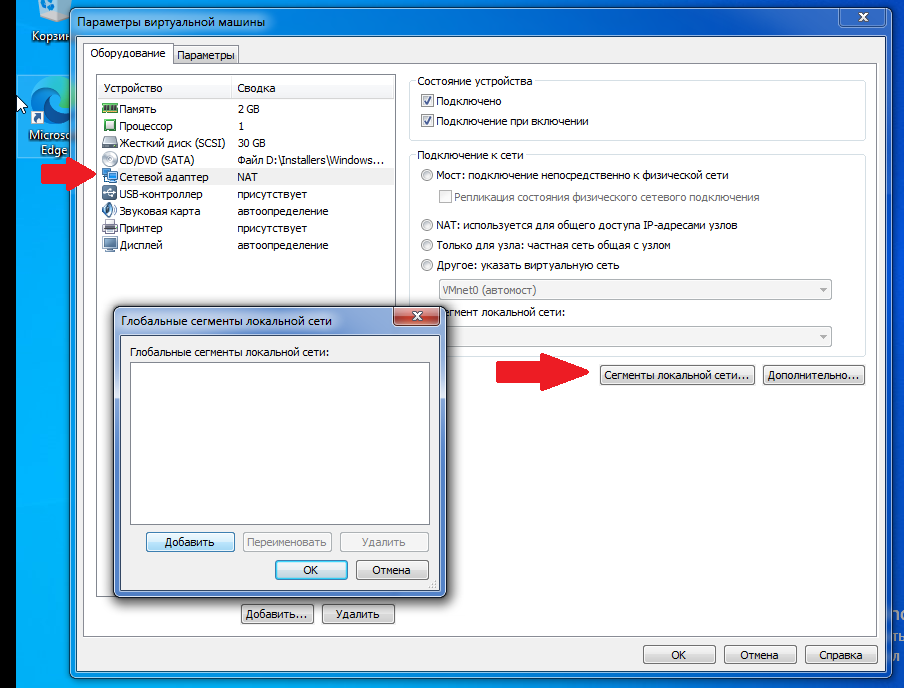
\includegraphics[scale=0.6]{_2}}
		\label{fig:image}
	\end{figure}

	\clearpage

	Добавьте новый сегмент "SRV1-CLI1".
	
	\begin{figure}[h]
		\center{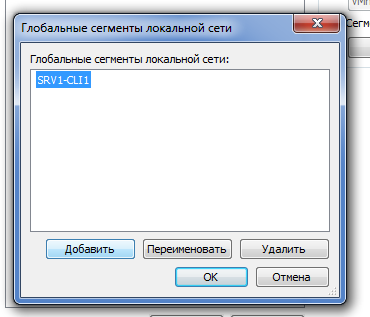
\includegraphics[scale=0.6]{_3}}
		\label{fig:image}
	\end{figure}

	В настройках обеих виртуальных машин укажите сегмент локальной сети "SRV1-CLI1"
	
	\begin{figure}[h]
		\center{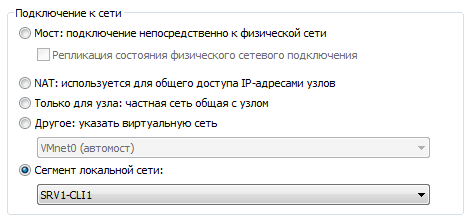
\includegraphics[scale=0.6]{_4}}
		\label{fig:image}
	\end{figure}

	\clearpage
	
	\subsection{Настройка SRV1}
	
	Настройка имени хоста, ip адреса, DHCP и контроллера домена.
	
	\subsubsection{Смена имени хоста}
	
	Панель управления -> Система -> Свойства системы
	
	\begin{figure}[h]
		\center{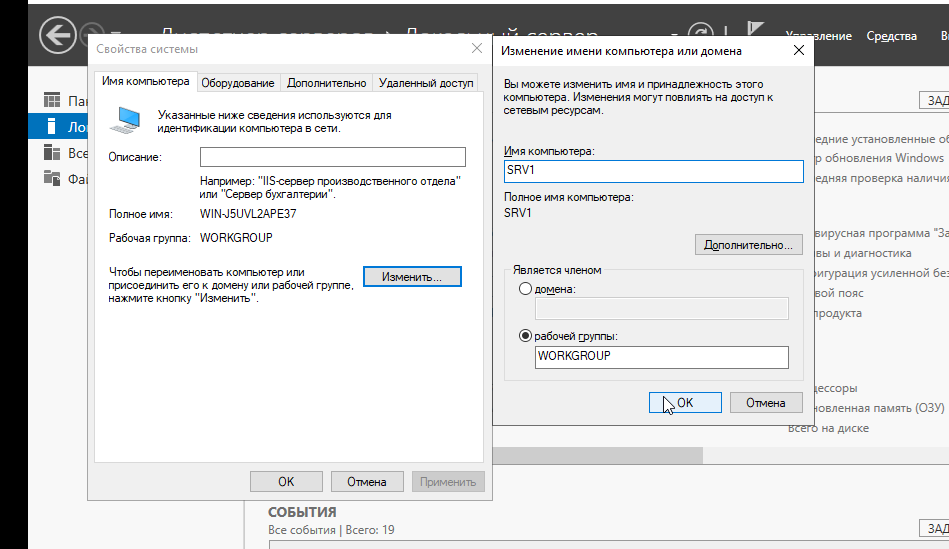
\includegraphics[scale=0.6]{1}}
		\label{fig:image}
	\end{figure}

	\clearpage

	\subsubsection{Смена ip адреса}
	
	Панель управления -> Сеть и интернет -> Сетевые подключения
	
	\begin{figure}[h]
		\center{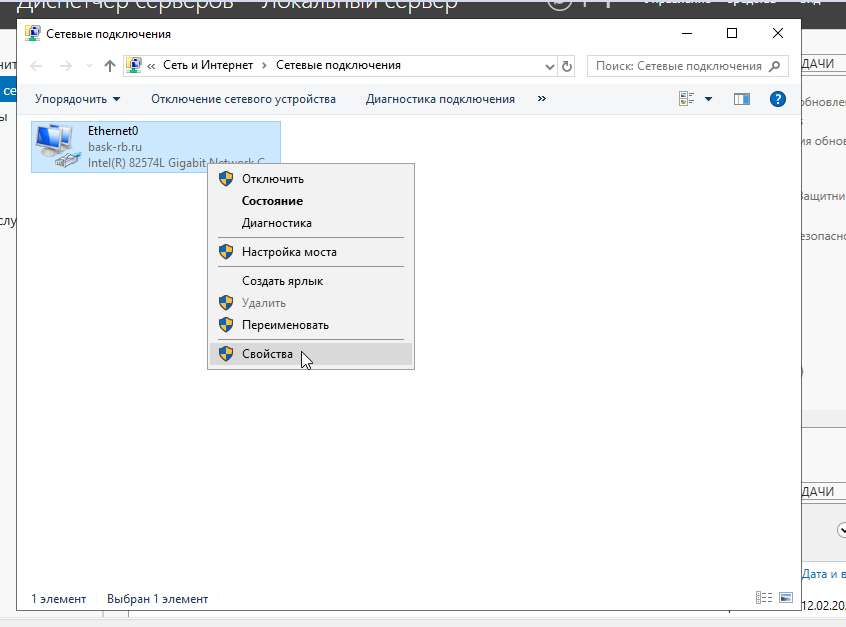
\includegraphics[scale=0.5]{17}}
		\label{fig:image}
	\end{figure}

	\begin{figure}[h]
		\center{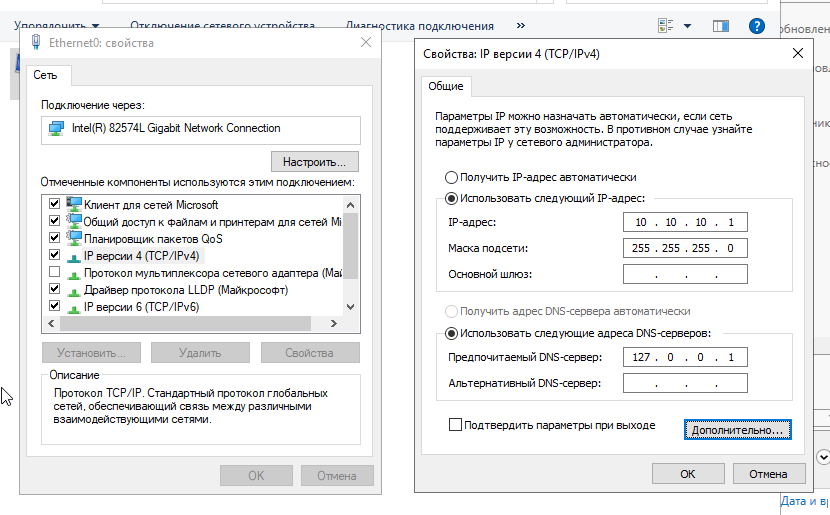
\includegraphics[scale=0.5]{18}}
		\label{fig:image}
	\end{figure}

	\clearpage
	
	\subsubsection{Создание контроллера домена}
	
	Контроллер домена - это серверный компьютер , который отвечает на запросы аутентификации безопасности (вход в систему и т. Д.) В пределах домена Windows . Домен - это концепция, представленная в Windows NT, посредством которой пользователю может быть предоставлен доступ к ряду компьютерных ресурсов с использованием единой комбинации имени пользователя и пароля.
	
	Чтобы создать контроллер домена, перейдите по пути: Диспетчер серверов -> Управление -> Добавить роли и компоненты
	
	Выберете сервер SRV1 в списке и добавьте следующие роли:
	
	\begin{figure}[h]
		\center{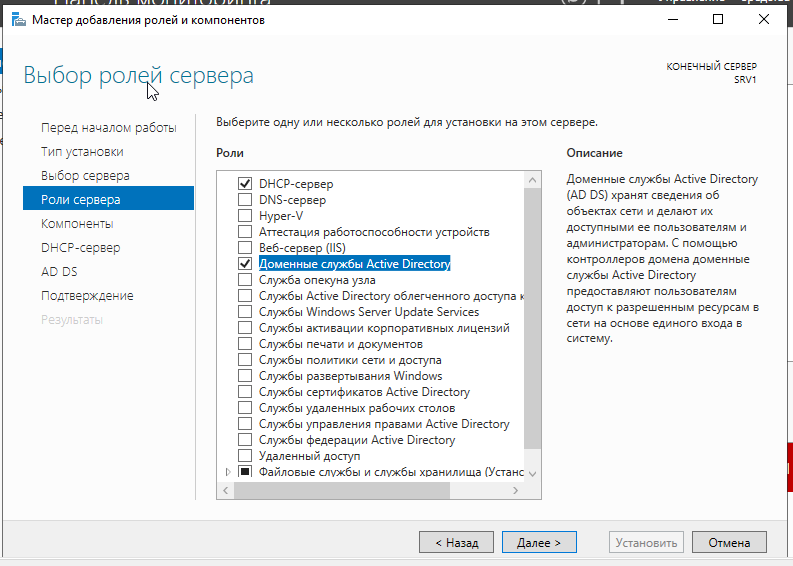
\includegraphics[scale=0.5]{2}}
		\label{fig:image}
	\end{figure}

	\clearpage

	В панели уведомлений выберете "Повысить роль этого сервера до уровня контроллера":
	
	\begin{figure}[h]
		\center{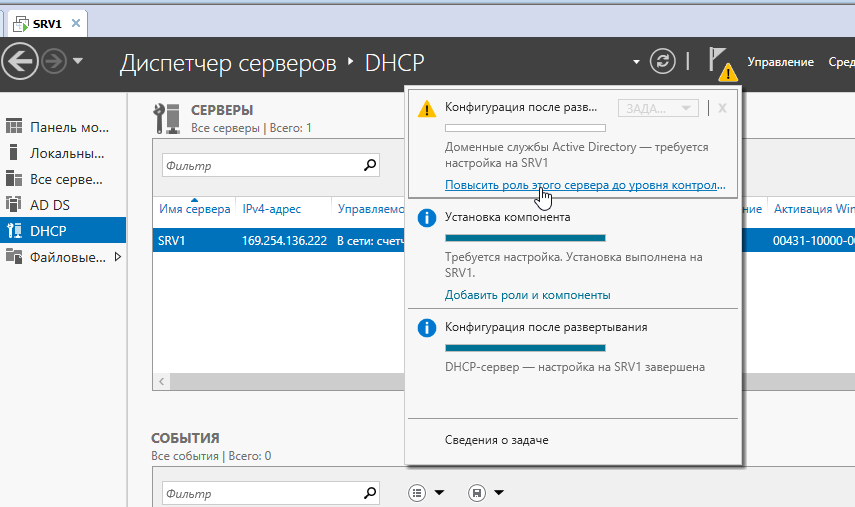
\includegraphics[scale=0.5]{5}}
		\label{fig:image}
	\end{figure}

	Заполните данные по примеру:
	
	\begin{figure}[h]
		\center{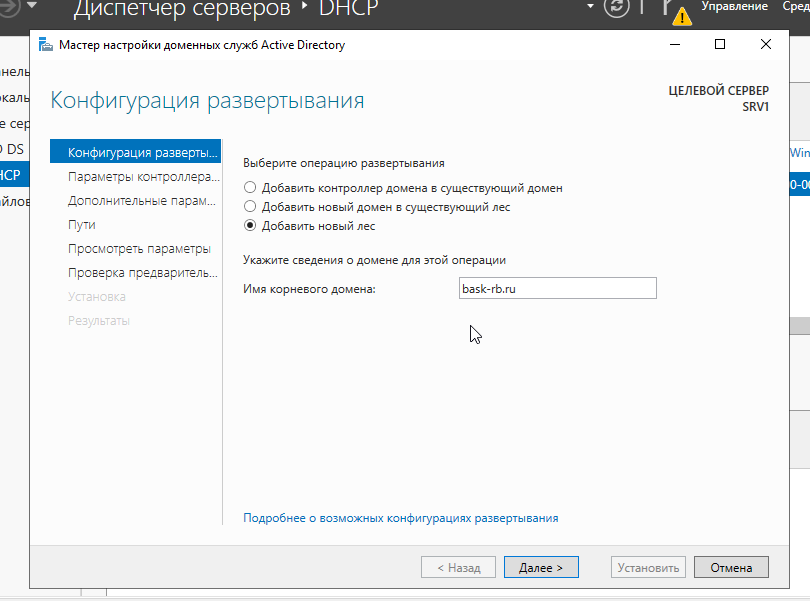
\includegraphics[scale=0.5]{6}}
		\label{fig:image}
	\end{figure}

	\begin{figure}[h]
		\center{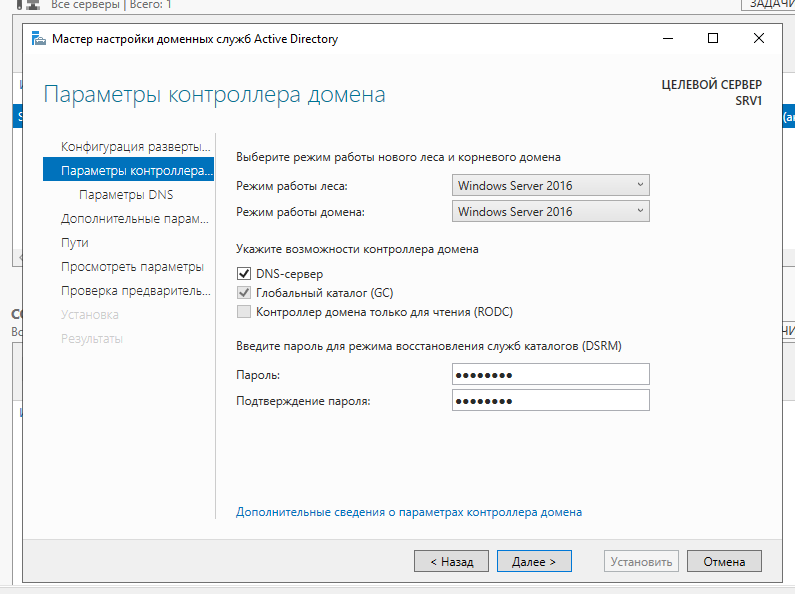
\includegraphics[scale=0.5]{7}}
		\label{fig:image}
	\end{figure}

	\begin{figure}[h]
		\center{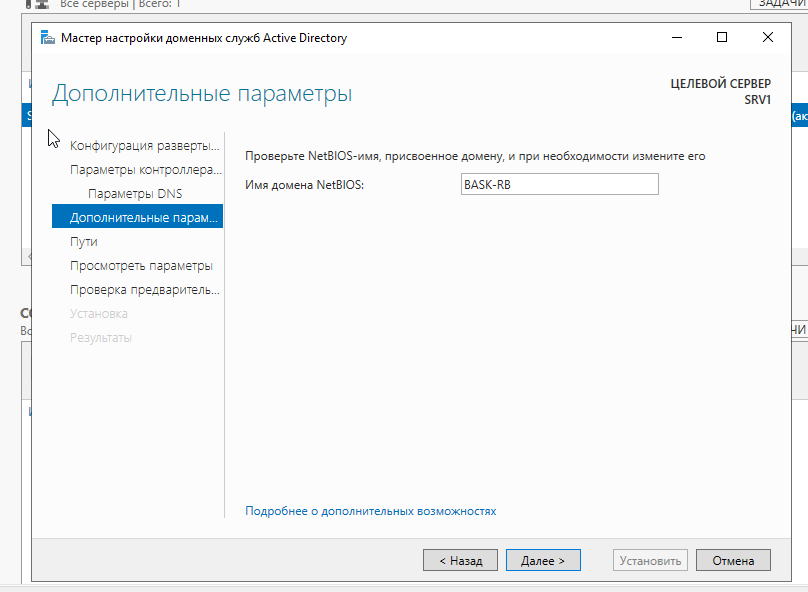
\includegraphics[scale=0.5]{8}}
		\label{fig:image}
	\end{figure}

	\begin{figure}[h]
		\center{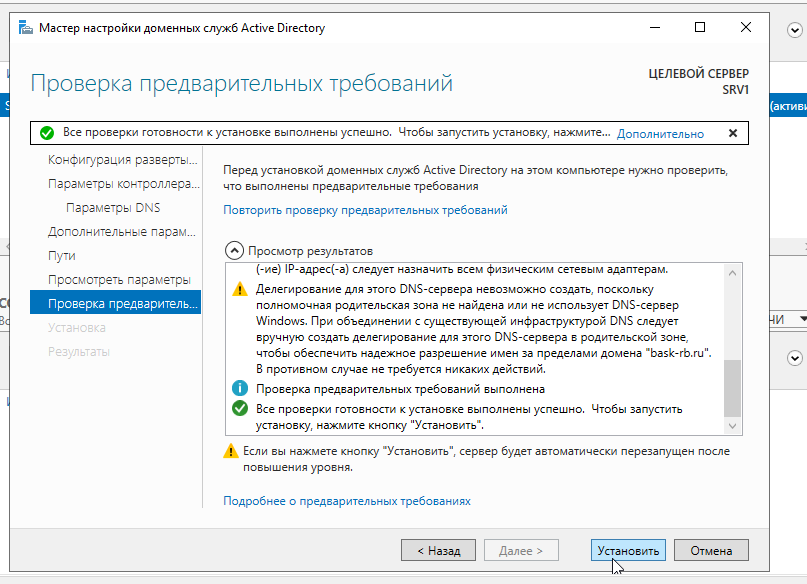
\includegraphics[scale=0.5]{9}}
		\label{fig:image}
	\end{figure}

	\clearpage
	
	\subsubsection{Создание пользователя}
	
	\begin{figure}[h]
		\center{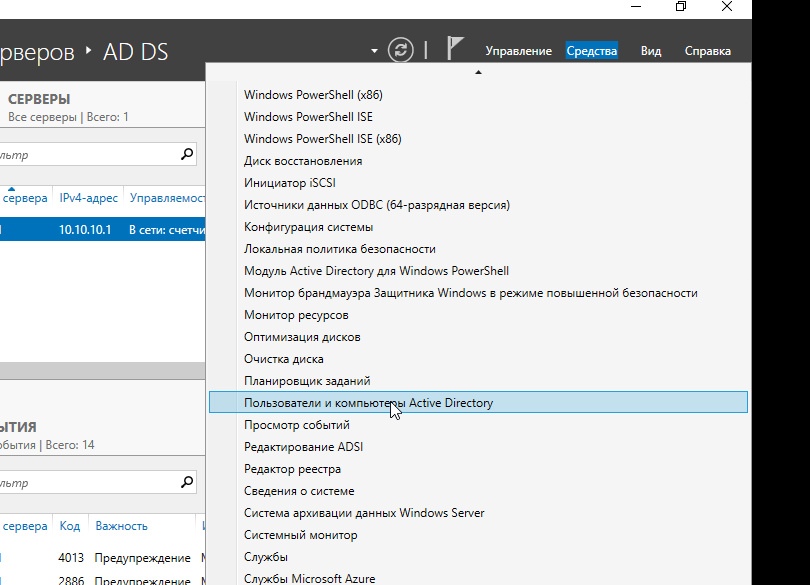
\includegraphics[scale=0.5]{21}}
		\label{fig:image}
	\end{figure}

	В корневом каталоге домена создайте подразделение bask
	
	\begin{figure}[h]
		\center{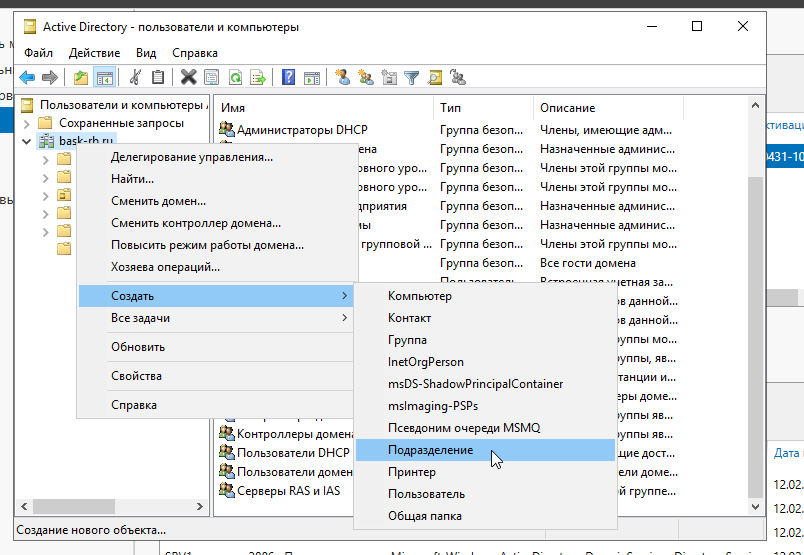
\includegraphics[scale=0.5]{22}}
		\label{fig:image}
	\end{figure}

	\clearpage

	\begin{figure}[h]
		\center{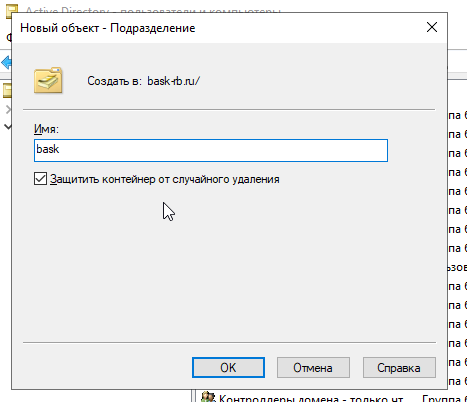
\includegraphics[scale=0.7]{23}}
		\label{fig:image}
	\end{figure}

	В этом подразделении создайте пользователя:

	\begin{figure}[h]
		\center{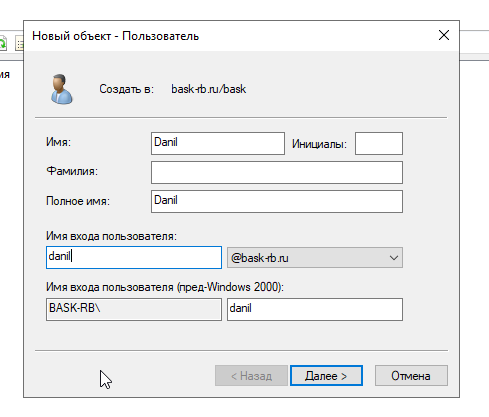
\includegraphics[scale=0.7]{24}}
		\label{fig:image}
	\end{figure}
	
	\clearpage
	
	\subsubsection{Настройка DHCP}
	
	DHCP — сетевой протокол, позволяющий сетевым устройствам автоматически получать IP-адрес и другие параметры, необходимые для работы в сети TCP/IP. Данный протокол работает по модели «клиент-сервер».
	
	Перед настройкой должна быть установлена роль \textbf{«DHCP-сервер»}, которую мы установили перед настройкой контроллера домена.
	
	Перейдите по пути: Диспетчер серверов -> Средства -> DHCP и заполните по инструкции:
	
	\begin{figure}[h]
		\center{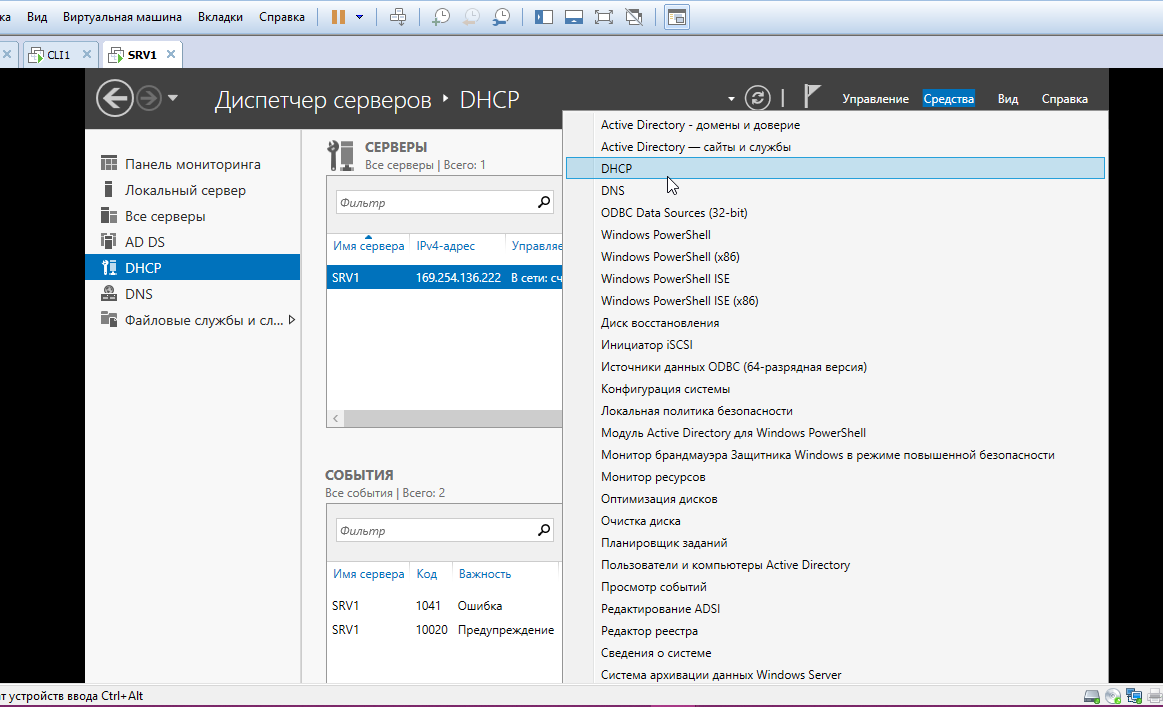
\includegraphics[scale=0.5]{10}}
		\label{fig:image}
	\end{figure}

	\begin{figure}[h]
		\center{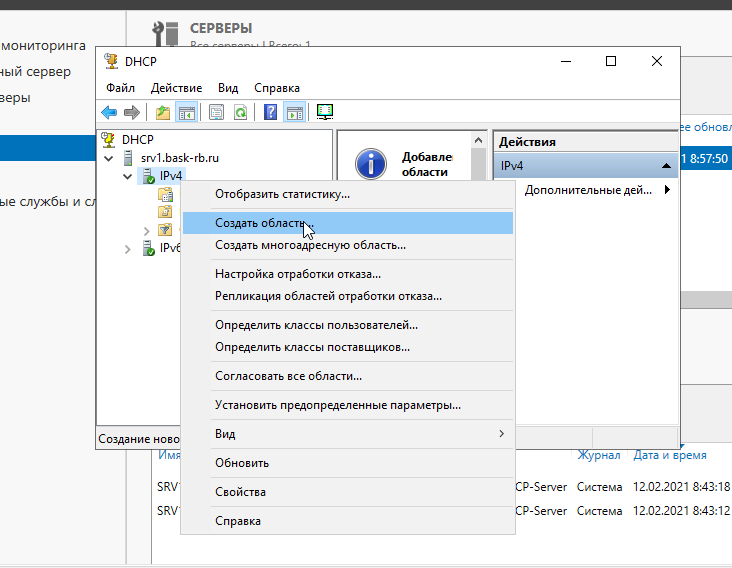
\includegraphics[scale=0.5]{11}}
		\label{fig:image}
	\end{figure}

	\begin{figure}[h]
		\center{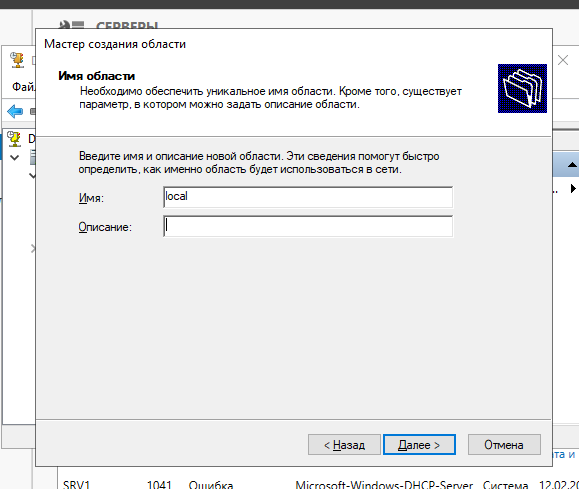
\includegraphics[scale=0.6]{12}}
		\label{fig:image}
	\end{figure}
	
	\begin{figure}[h]
		\center{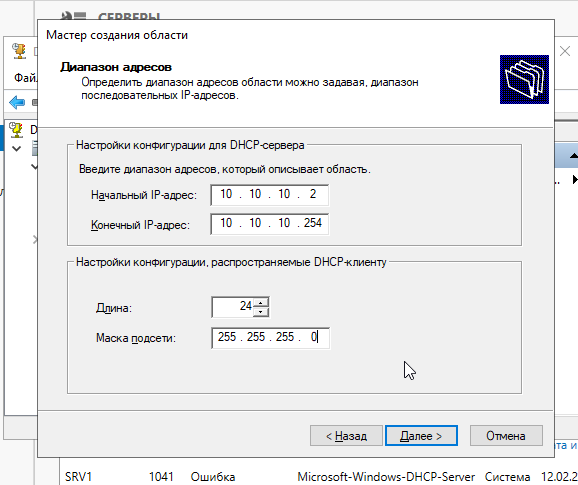
\includegraphics[scale=0.6]{13}}
		\label{fig:image}
	\end{figure}
	
	\begin{figure}[h]
		\center{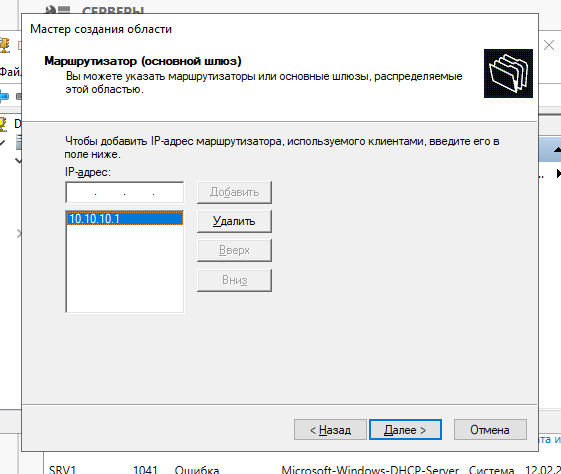
\includegraphics[scale=0.6]{14}}
		\label{fig:image}
	\end{figure}
	
	\begin{figure}[h]
		\center{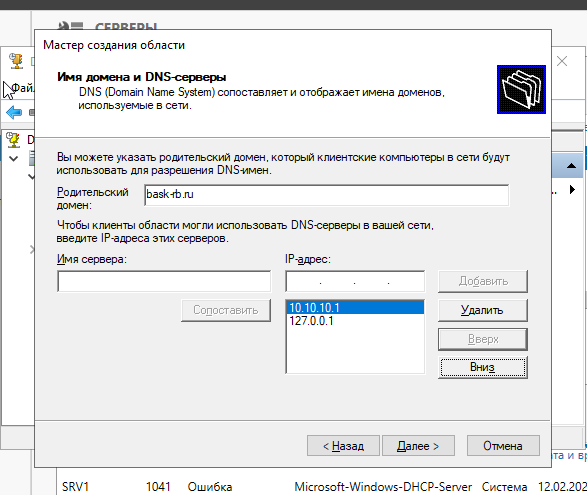
\includegraphics[scale=0.6]{15}}
		\label{fig:image}
	\end{figure}
	
	\begin{figure}[h]
		\center{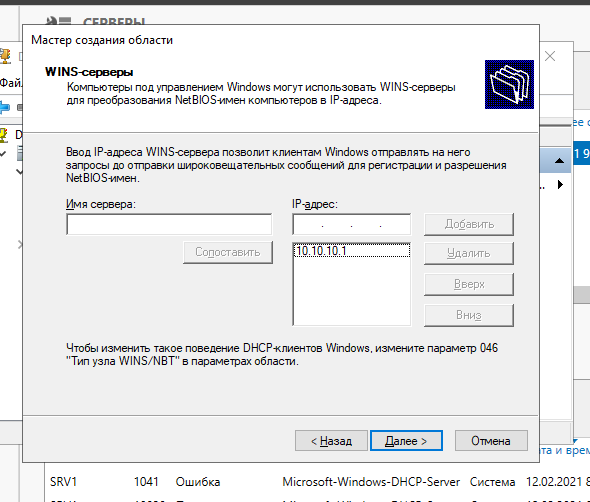
\includegraphics[scale=0.6]{16}}
		\label{fig:image}
	\end{figure}

	\clearpage
	
	Авторизация DHCP сервера:

	\begin{figure}[h]
		\center{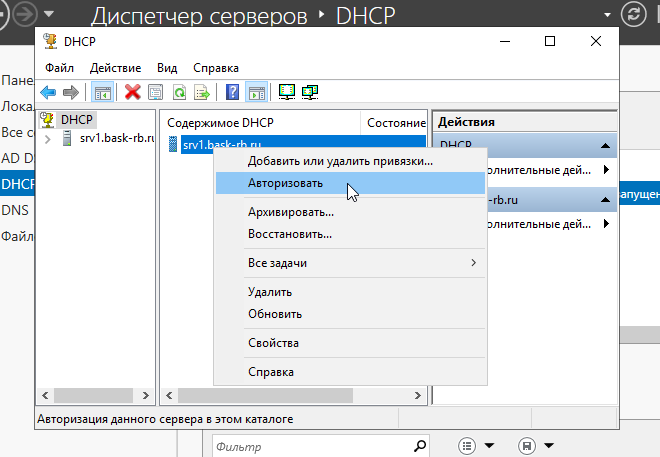
\includegraphics[scale=0.6]{20}}
		\label{fig:image}
	\end{figure}

	\clearpage

	\subsection{Настройка CLI1}
	
	\subsubsection{Настройка имени хоста и авторизация в домене}
	
	\begin{figure}[h]
		\center{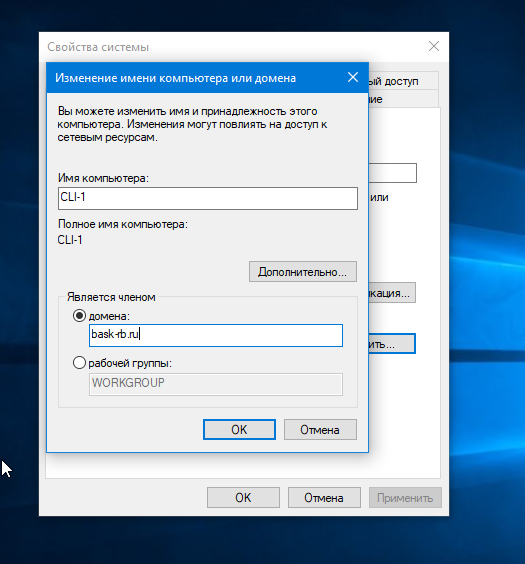
\includegraphics[scale=1]{19}}
		\label{fig:image}
	\end{figure}

	\clearpage
	
	Введите логин и пароль от аккаунта, который мы создали в домене bask-rb.ru:

	\begin{figure}[h]
		\center{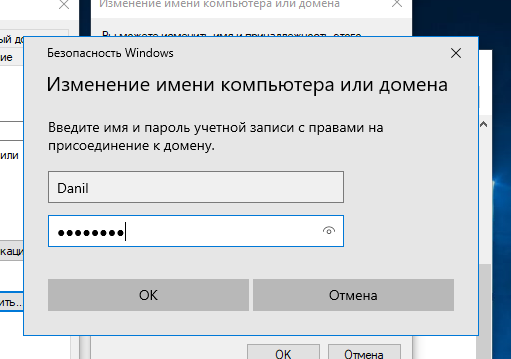
\includegraphics[scale=0.5]{26}}
		\label{fig:image}
	\end{figure}

	Проверка протокола ICMP:
	
	\begin{figure}[h]
		\center{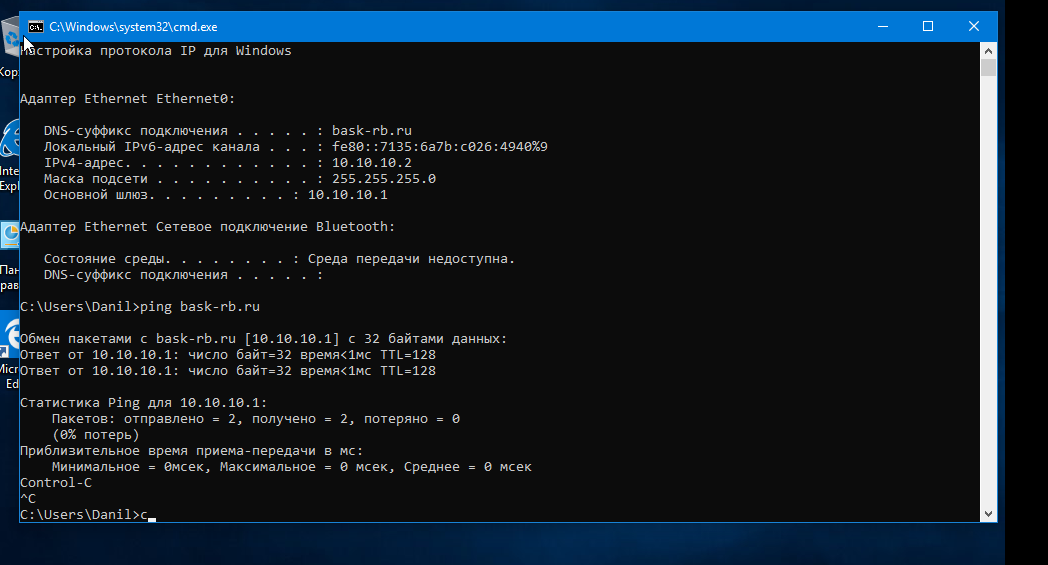
\includegraphics[scale=0.6]{27}}
		\label{fig:image}
	\end{figure}


\end{document}